%%%%%%%%%%%%  Generated using docx2latex.com  %%%%%%%%%%%%%%

%%%%%%%%%%%%  v2.0.0-beta  %%%%%%%%%%%%%%

\documentclass[12pt]{article}
\usepackage{amsmath}
\usepackage{latexsym}
\usepackage{amsfonts}
\usepackage[normalem]{ulem}
\usepackage{soul}
\usepackage{array}
\usepackage{amssymb}
\usepackage{extarrows}
\usepackage{graphicx}
\usepackage[backend=biber,
style=numeric,
sorting=none,
isbn=false,
doi=false,
url=false,
]{biblatex}\addbibresource{bibliography.bib}

\usepackage{subfig}
\usepackage{wrapfig}
\usepackage{wasysym}
\usepackage{enumitem}
\usepackage{adjustbox}
\usepackage{ragged2e}
\usepackage[svgnames,table]{xcolor}
\usepackage{tikz}
\usepackage{longtable}
\usepackage{changepage}
\usepackage{setspace}
\usepackage{hhline}
\usepackage{multicol}
\usepackage{tabto}
\usepackage{float}
\usepackage{multirow}
\usepackage{makecell}
\usepackage{fancyhdr}
\usepackage[toc,page]{appendix}
\usepackage[hidelinks]{hyperref}
\usetikzlibrary{shapes.symbols,shapes.geometric,shadows,arrows.meta}
\tikzset{>={Latex[width=1.5mm,length=2mm]}}
\usepackage{flowchart}\usepackage[paperheight=11.0in,paperwidth=8.5in,left=1.0in,right=1.0in,top=1.0in,bottom=1.0in,headheight=1in]{geometry}
\usepackage[utf8]{inputenc}
\usepackage[T1]{fontenc}
\TabPositions{0.5in,1.0in,1.5in,2.0in,2.5in,3.0in,3.5in,4.0in,4.5in,5.0in,5.5in,6.0in,}

\urlstyle{same}


 %%%%%%%%%%%%  Set Depths for Sections  %%%%%%%%%%%%%%

% 1) Section
% 1.1) SubSection
% 1.1.1) SubSubSection
% 1.1.1.1) Paragraph
% 1.1.1.1.1) Subparagraph


\setcounter{tocdepth}{5}
\setcounter{secnumdepth}{5}


 %%%%%%%%%%%%  Set Depths for Nested Lists created by \begin{enumerate}  %%%%%%%%%%%%%%


\setlistdepth{9}
\renewlist{enumerate}{enumerate}{9}
		\setlist[enumerate,1]{label=\arabic*)}
		\setlist[enumerate,2]{label=\alph*)}
		\setlist[enumerate,3]{label=(\roman*)}
		\setlist[enumerate,4]{label=(\arabic*)}
		\setlist[enumerate,5]{label=(\Alph*)}
		\setlist[enumerate,6]{label=(\Roman*)}
		\setlist[enumerate,7]{label=\arabic*}
		\setlist[enumerate,8]{label=\alph*}
		\setlist[enumerate,9]{label=\roman*}

\renewlist{itemize}{itemize}{9}
		\setlist[itemize]{label=$\cdot$}
		\setlist[itemize,1]{label=\textbullet}
		\setlist[itemize,2]{label=$\circ$}
		\setlist[itemize,3]{label=$\ast$}
		\setlist[itemize,4]{label=$\dagger$}
		\setlist[itemize,5]{label=$\triangleright$}
		\setlist[itemize,6]{label=$\bigstar$}
		\setlist[itemize,7]{label=$\blacklozenge$}
		\setlist[itemize,8]{label=$\prime$}

\setlength{\topsep}{0pt}\setlength{\parindent}{0pt}

 %%%%%%%%%%%%  This sets linespacing (verticle gap between Lines) Default=1 %%%%%%%%%%%%%%


\renewcommand{\arraystretch}{1.3}


%%%%%%%%%%%%%%%%%%%% Document code starts here %%%%%%%%%%%%%%%%%%%%



\begin{document}
\begin{Center}
{\fontsize{16pt}{19.2pt}\selectfont \textbf{Analysis based on H1\_B Visa petition data and approval prediction}\par}
\end{Center}\par

\begin{Center}
{\fontsize{14pt}{16.8pt}\selectfont ORIE4741: Chengnan Xu(cx223), Tian Yu(ty364)\par}
\end{Center}\par


\vspace{\baselineskip}
{\fontsize{14pt}{16.8pt}\selectfont \textbf{1. Problem definition}\par}\par

\begin{justify}
In our project, we want to predict the outcome of H1B\_visa applicants based on the dataset. H1\_B visa, non-immigration visa category for international students who want to work in America, is highly desired. It required petition employees at least a bachelor’s degree. As more and more employees go into America, based on Citizenship and Immigration Services(USCIS) grants 85,000 H1\_B visas[1] every year, the visa outcome for the applicants is of importance. 
\end{justify}\par

\begin{justify}
The input to our algorithm is based on the dataset features and we will also do some feature engineering such as converted to 0 or 1 for the feature. The output would be the case status whether certified or denied.
\end{justify}\par


\vspace{\baselineskip}
{\fontsize{14pt}{16.8pt}\selectfont \textbf{2. About the dataset}\par}\par

\textbf{2.1 Dataset overview}\par

\begin{justify}
Our columns features were divided into 2 types: 6 nominal variables, 4 continuous features and Our dataset is from Kaggle listed under the name $``$H-1B Visa Petitions 2011-2016 dataset$"$ . There are 10 features and more than 3 million examples in our dataset. The columns in the dataset include case status, employer name, worksite coordinates, job title, prevailing wage, occupation code, and year filed. The dataset contains some missing data and the data values are heterogeneous including continuous values, discrete values, nominal data and text. 
\end{justify}\par



%%%%%%%%%%%%%%%%%%%% Figure/Image No: 1 starts here %%%%%%%%%%%%%%%%%%%%

\begin{figure}[H]
	\begin{Center}
		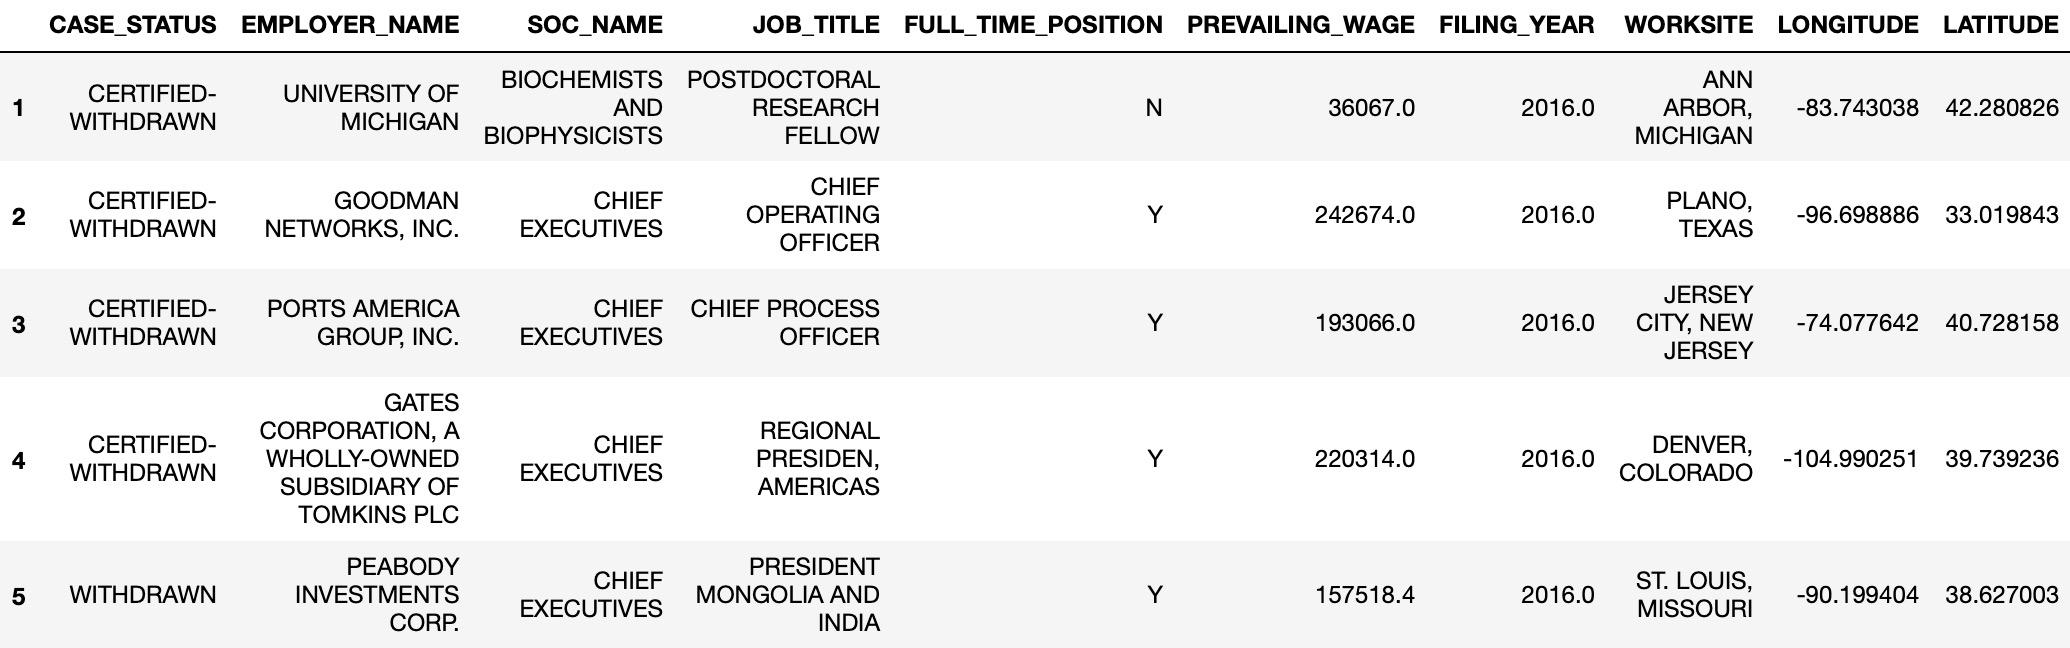
\includegraphics[width=6.28in,height=1.97in]{./media/image3.jpg}
	\end{Center}
\end{figure}


%%%%%%%%%%%%%%%%%%%% Figure/Image No: 1 Ends here %%%%%%%%%%%%%%%%%%%%

\begin{justify}
 
\end{justify}\par

\begin{Center}
{\fontsize{8pt}{9.6pt}\selectfont Table.1\  First 5 points from the unprocessed dataset\par}
\end{Center}\par


\vspace{\baselineskip}
\begin{justify}
\textbf{2.2 Dataset Characteristics}
\end{justify}\par

\begin{justify}
We\ processed some of the existing features, created new features that we thought could be useful for prediction and discarded some features using the library Pandas. For example, in our training data, some original features like SOC NAME  is not directly related to our CASE\_STATUS, Therefore, we calculated the success rate and total number of applications to create new highly correlated features The detailed explanation is below.
\end{justify}\par

\begin{justify}
CASE\_STATUS: We only maintain ‘CERTIFIED’ and ‘DENIED’ in CASE\_STATUS, with labeled as ‘1’ and ‘0’.
\end{justify}\par

\begin{justify}
FULL\_TIME\_POSITION: For the full time position column, there are two cases, $ \{ $ Y, N$ \} $  for applicants who have full time position or not. We labeled $``$FULL TIME POSITION$"$  = $``$Y$"$  as 1 and $``$FULL TIME POSITION$"$  = $``$N$"$  as 0.
\end{justify}\par

\begin{justify}
EMPLOYER\_ACCEPTANCE:\  We created a feature for the ratio of H-1B applicants who were certified per employer. 
\end{justify}\par

\begin{justify}
EMPLOYER\_ACCEPTANCE: Also categorized into six types for ratio of acceptance and converted the data into one-hot-k representation. We created a feature for the success rate per SOC type,converted to one-hot-k representation.
\end{justify}\par

\begin{justify}
JOB\_ACCEPTANCE: We created a feature for the success rate per Job type, converted to one-hot-k representation.
\end{justify}\par

\begin{justify}
WORKSITE:\ For the format of $ \{ $ City, State$ \} $ ,  we only included $"$ State$"$  and converted the data into one-hot-k representation.
\end{justify}\par

\begin{justify}
WAGE\_CATEGRORY: we created a feature for the prevailing wage which is the average wage paid to employees with similar qualifications. Category the average wage into five kinds$ \{ $ very low, low, medium, high, very high$ \} $  and then converted to one-hot-k representation. 
\end{justify}\par

\begin{justify}
FILING\_YEAR:\ \ columns Year the applicants were filed,  we converted data of different year into type int and applied one-hot-k representation.
\end{justify}\par

\begin{justify}
\textbf{2.3 Data Exploration}
\end{justify}\par

\begin{justify}
Our label CASE\_STATUS has seven different categories. To get more information about the CASE\_STATUS, we plot the histogram of case status versus number of petition of the visa petition. 
\end{justify}\par



%%%%%%%%%%%%%%%%%%%% Figure/Image No: 2 starts here %%%%%%%%%%%%%%%%%%%%

\begin{figure}[H]
	\begin{Center}
		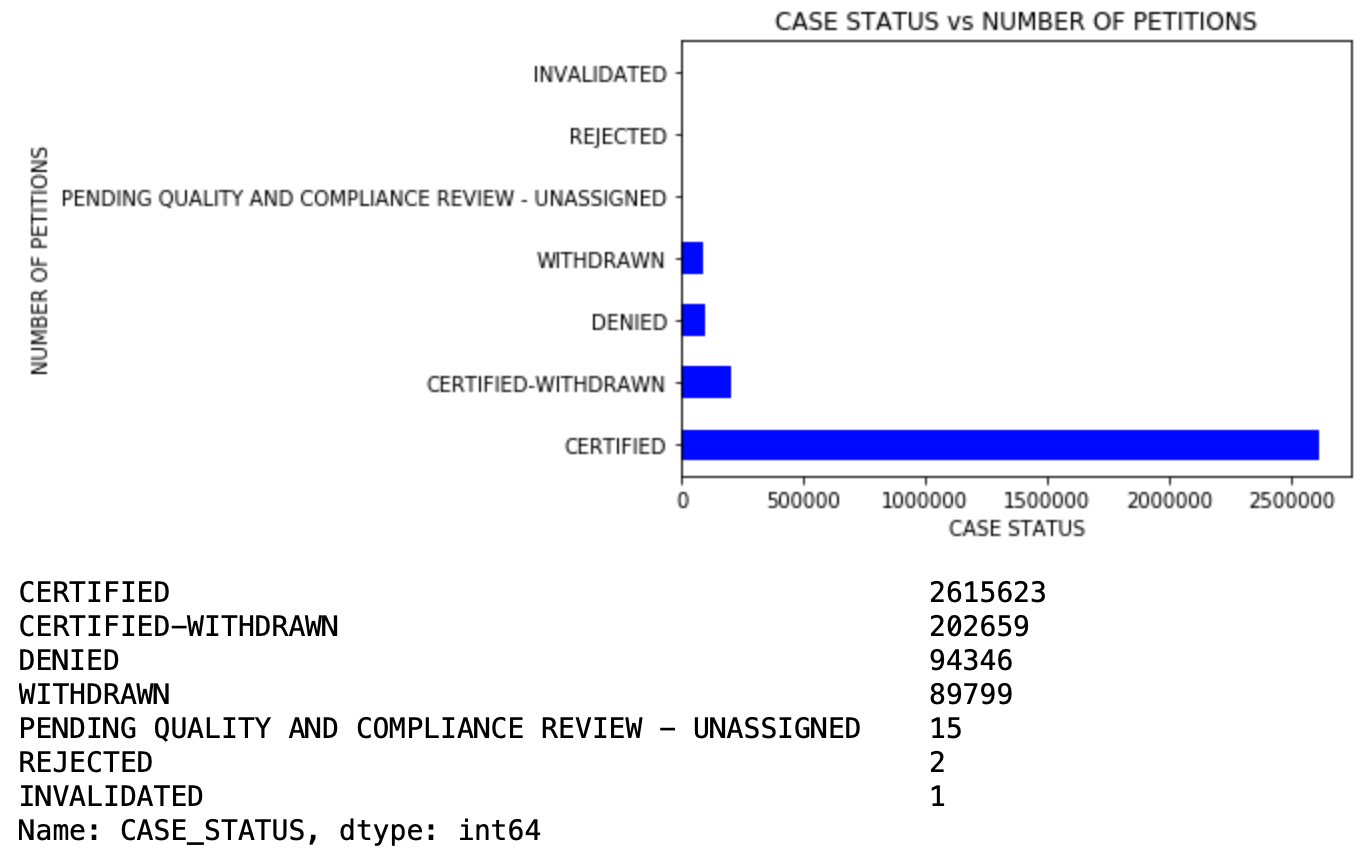
\includegraphics[width=4.89in,height=1.98in]{./media/image2.png}
	\end{Center}
\end{figure}


%%%%%%%%%%%%%%%%%%%% Figure/Image No: 2 Ends here %%%%%%%%%%%%%%%%%%%%

\par

\begin{Center}
{\fontsize{8pt}{9.6pt}\selectfont Fig. 1.1 the histogram of seven classes in CASE\_STATUS\par}
\end{Center}\par


\vspace{\baselineskip}


%%%%%%%%%%%%%%%%%%%% Figure/Image No: 3 starts here %%%%%%%%%%%%%%%%%%%%


\begin{figure}[H]	\begin{subfigure}		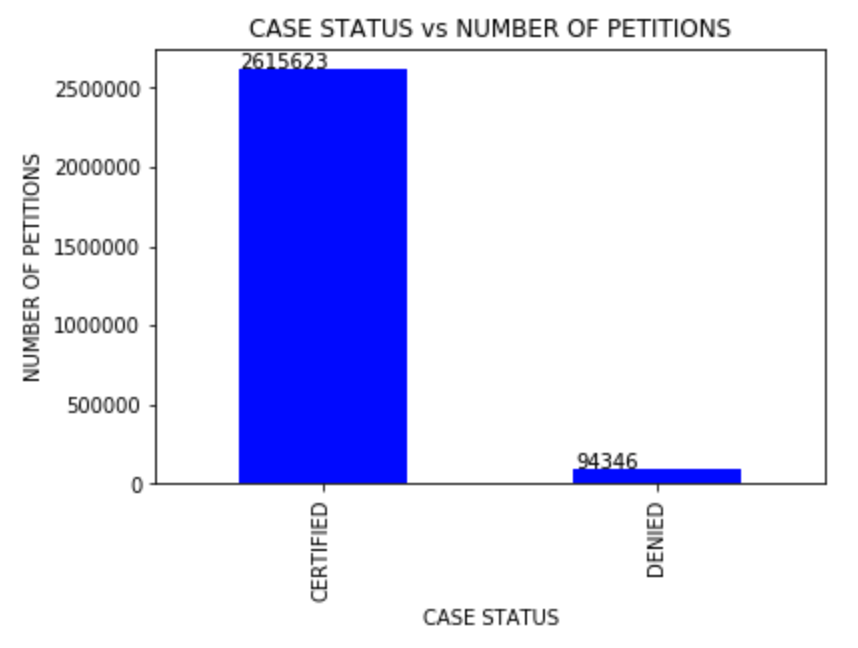
\includegraphics[width=0.45\textwidth]{./media/image1.png}
	\end{subfigure}
~	\begin{subfigure}		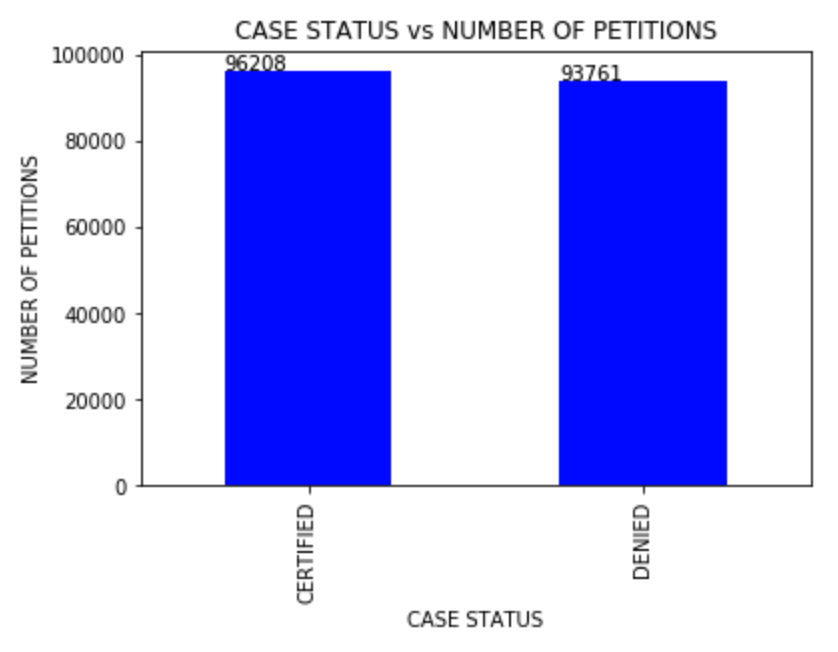
\includegraphics[width=0.45\textwidth]{./media/image4.png}
	\end{subfigure}
~
\end{figure}


%%%%%%%%%%%%%%%%%%%% Figure/Image No: 3 Ends here %%%%%%%%%%%%%%%%%%%%

\par

{\fontsize{8pt}{9.6pt}\selectfont \ \ \ \ \ \ \ \ \ \ \ Fig.1.2  imbalanced classes in CASE\_STATUS{\fontsize{10pt}{12.0pt}\selectfont \tab \ \ \ \ \ \ \ \ \ \ \ \ \ \ \ \ \ \  {\fontsize{8pt}{9.6pt}\selectfont  Fig.1.3 equal ratio after undersampling\par}\par}\par}\par


\vspace{\baselineskip}
\begin{justify}
From\ Fig.1, we observe that the total amount of some CASE\_STATUS outcome classes are relevant quite low. We decided to discard the ‘INVALIDATED,’ ‘REJECTED’, ‘PENDING QUALITY AND COMPLIANCE REVIEW - UNASSIGNED’ class because of the trivial amount.  
\end{justify}\par

\begin{justify}
Then\ I compute the top employers sponsoring H1’B, we can see the top are indians’ company which maybe they want to  hire more technique people to increase companies’ profits. 
\end{justify}\par


\vspace{\baselineskip}


%%%%%%%%%%%%%%%%%%%% Figure/Image No: 4 starts here %%%%%%%%%%%%%%%%%%%%

\begin{figure}[H]
	\begin{Center}
		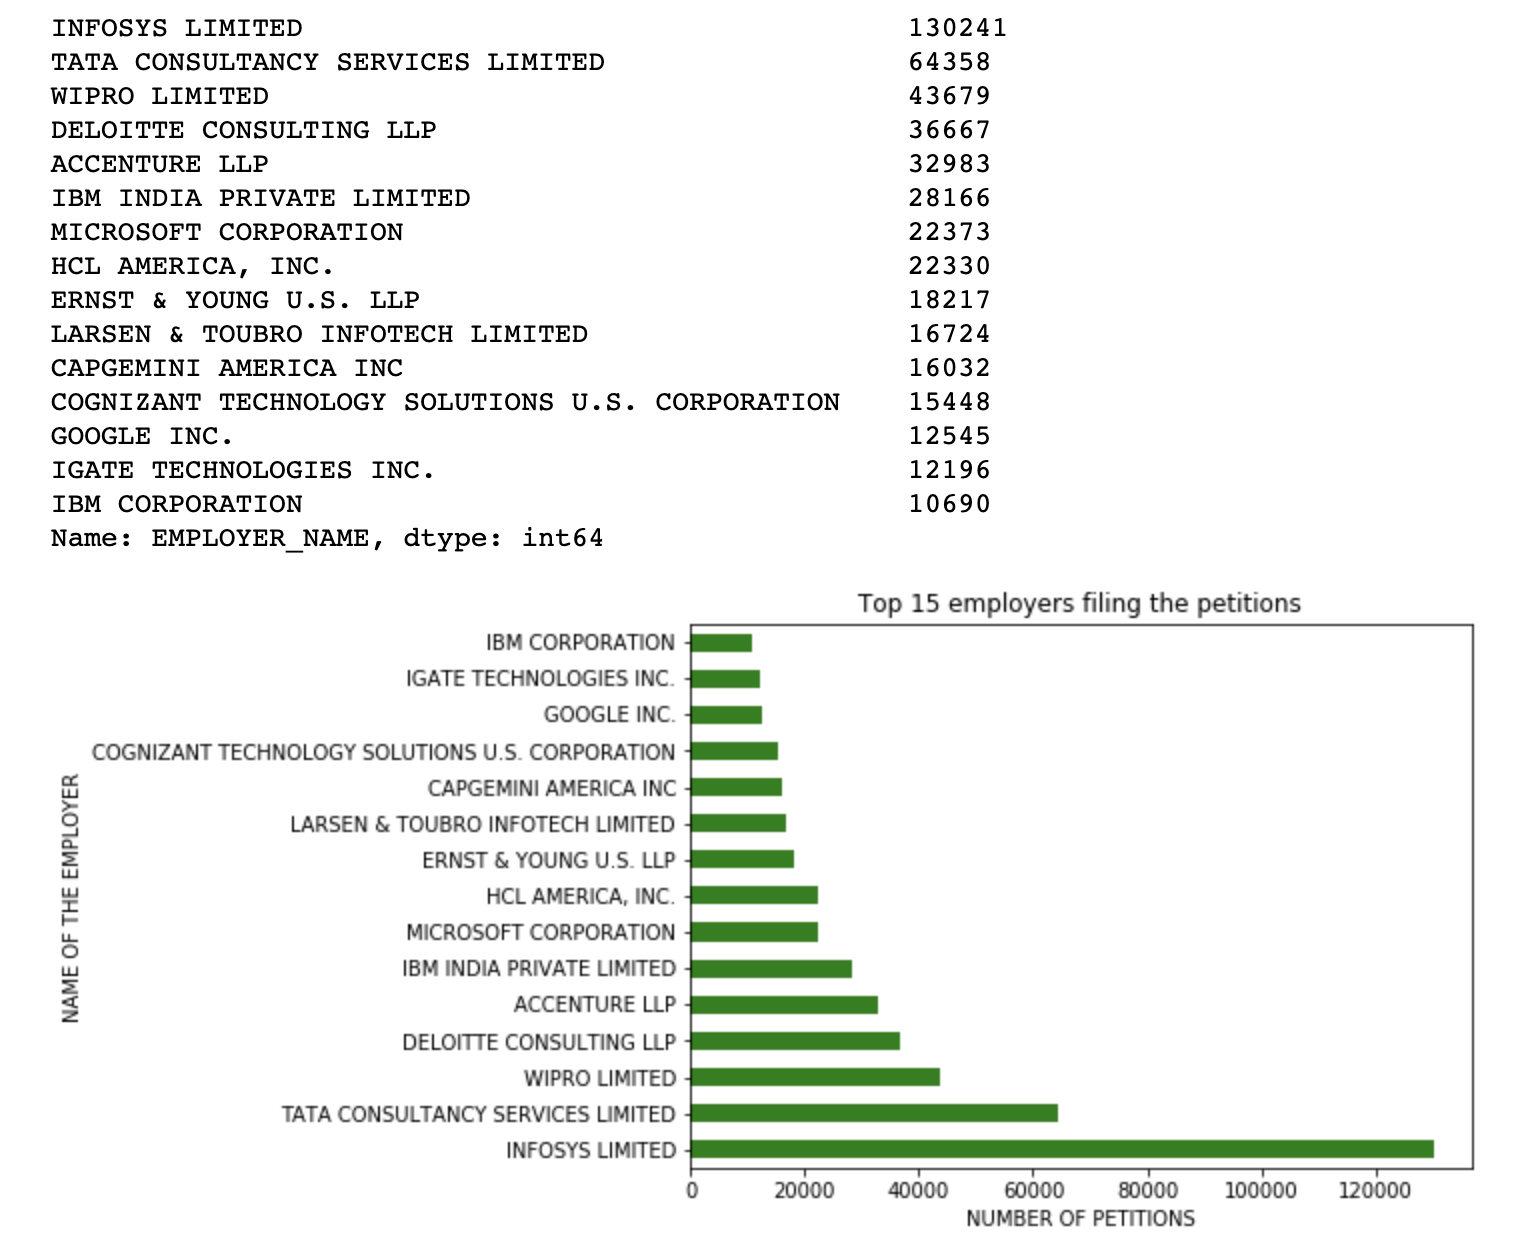
\includegraphics[width=6.5in,height=2.85in]{./media/image11.png}
	\end{Center}
\end{figure}


%%%%%%%%%%%%%%%%%%%% Figure/Image No: 4 Ends here %%%%%%%%%%%%%%%%%%%%

\par

\begin{Center}
{\fontsize{8pt}{9.6pt}\selectfont Figure 2 Top employers sponsoring H1-B\par}
\end{Center}\par


\vspace{\baselineskip}
\begin{justify}
\textbf{2.4 Cleaning the Data}
\end{justify}\par

\begin{justify}
As with any dataset, there were many missing values. By applying pandas.dataframe.isnull(), we statistically summarized the missing data in the dataset and we remove rows with null values for $``$EMPLOYER\_NAME$"$ , $``$SOC\_NAME$"$ , $``$JOB\_TITLE$"$ , $``$FULL\_TIME\_POSITION$"$ , $``$PREVAILING\_WAGE$"$  by applying dataframe.dropna. The missing data is like Employer) name is missing about 20 numbers, Job title is about 0, full\_time\_position is about 1, the prevailing wage is about more than 50;
\end{justify}\par

\begin{justify}
We also plot the histogram of CASE\_STATUS vs number of petitions. From Fig.2.1, we can see the dataset is highly imbalanced, with only 3.5$\%$  of case status being declined. The imbalanced dataset may contribute to model’s overfitting problem, the problem and solution will be elaborated in the preliminary models part.
\end{justify}\par

\begin{justify}
After the pre-processing steps described above, we split the training and test sets 80:20. Training set had a total of 2.4 million examples. Due to the inherent bias in our dataset towards the $"$ CERTIFIED$"$  label(Fig. 2.1), the model learning from class imbalanced training dataset performed badly in the test datatest. The precision of $``$CERTIFIED$"$  class is up to 95$\%$  while the precision of $``$DENIED$"$  class is lower than 50$\%$ . The model is overfitting.
\end{justify}\par

\begin{justify}
To address imbalanced classes problem, undersampling the majority class is a good choice, especially when we have millions of rows in our project dataset. Undersampling can be defined as removing some observations of the majority class and it can only be applied after splitting test and train set. After resampling, we have an equal ratio of ‘CERTIFIED’ data points to ‘DENIED’ data points(Fig. 2.2) , but a smaller quantity of data to train machine learning models on.
\end{justify}\par


\vspace{\baselineskip}
\begin{justify}
\textbf{2.5 Feature selection}
\end{justify}\par

\begin{justify}
Since the preprocessed dataset in one-hot-encoding format has too many features. We need to eliminate unimportant feature. We employ the RFE(Recursive Feature Elimination) function in sklearn. The operating principle of the RFE is as follows. First, the estimator is trained on the initial set of features and the importance of each feature is obtained. Then, the least important features are pruned from the current set of features. That procedure is recursively repeated on the pruned set until the desired number of features to select is eventually reached. By employing RFE, we finally use the features with key words of {\fontsize{10pt}{12.0pt}\selectfont 'EMPLOYER', 'FILING', 'FULL', 'JOB', 'SOC', 'WAGE', and 'WORKSITE'.\par}
\end{justify}\par


\vspace{\baselineskip}
{\fontsize{14pt}{16.8pt}\selectfont \textbf{3. Models}\par}\par

\textbf{3.1 Logistic regression}\par

\begin{justify}
Logistic regression is a statistical machine learning algorithm that classifies the data by considering outcome variables on extreme ends and tries makes a logarithmic line that distinguishes between them.
\end{justify}\par

\begin{justify}
The logistic regression is suitable for the classification scenario. It has the low calculation cost and very efficient in terms of time and memory requirements. However, this model has relatively low classification accuracy and not suitable for the dataset with missing data or large feature space. 
\end{justify}\par

\begin{justify}
In logistic regression, we mainly pay attention to the hyperparameter of C and class\_weight. A smaller of C values specify stronger regularization. And class\_weight of the ‘auto’ modeclass\_weight can over/undersample by given weights. 
\end{justify}\par

\begin{justify}
The confusion matrix of the logistic regression and result indicators are as follows.
\end{justify}\par



%%%%%%%%%%%%%%%%%%%% Figure/Image No: 5 starts here %%%%%%%%%%%%%%%%%%%%

\begin{figure}[H]
	\begin{Center}
		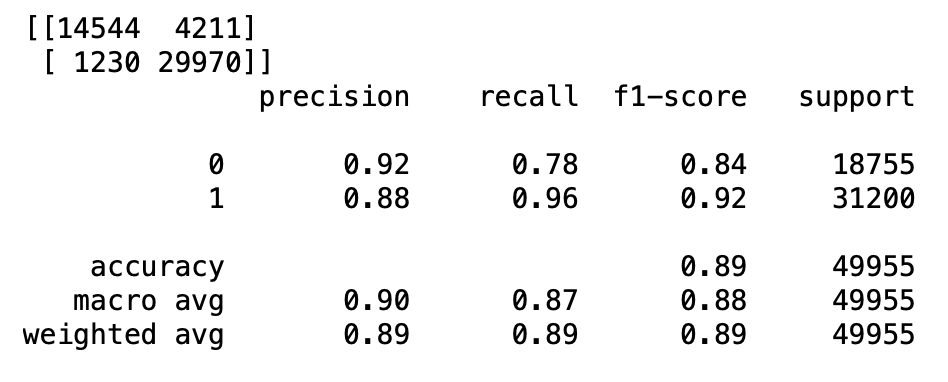
\includegraphics[width=3.3in,height=1.34in]{./media/image10.png}
	\end{Center}
\end{figure}


%%%%%%%%%%%%%%%%%%%% Figure/Image No: 5 Ends here %%%%%%%%%%%%%%%%%%%%

\par

\begin{Center}
{\fontsize{8pt}{9.6pt}\selectfont Figure.3 Confusion matrix and results indicators of logistic regression\par}
\end{Center}\par


\vspace{\baselineskip}
\textbf{3.2 Random forest classifier}\par

\begin{justify}
Random forest is an ensemble learning method for classification, regression and other tasks that operates by constructing a multitude of decision trees at training time and outputting the class that is the mode of the classification or mean prediction of the individual trees. There are several advantages​[2] of this method:
\end{justify}\par

\begin{justify}
●\  Small number of data loss does not change the regression model
\end{justify}\par

\begin{justify}
●\  The high generalization ability
\end{justify}\par

\begin{justify}
●\  Avoid the probability of overfitting
\end{justify}\par

\begin{justify}
●\  Do not need to choose the hyperparameters specifically
\end{justify}\par

\begin{justify}
For the random forest model, there are also some parameters that we need to consider:
\end{justify}\par

\begin{justify}
●\  Number of features: the quantity of features in the model
\end{justify}\par

\begin{justify}
●\  N estimators: the performance of the model
\end{justify}\par

\begin{justify}
●\  Min sample leaf: the ability of data capturing
\end{justify}\par

\begin{justify}
●\  Criterion: the validation criterion\\
While we implement the random forest model, we take the following values for our regression model to find the optimal prediction result. For the estimators, with the higher number of estimators can result in better performance in regression and prediction, but simultaneously, it can also bring the fact that the processing time will be much longer.
\end{justify}\par



%%%%%%%%%%%%%%%%%%%% Figure/Image No: 6 starts here %%%%%%%%%%%%%%%%%%%%

\begin{figure}[H]
	\begin{Center}
		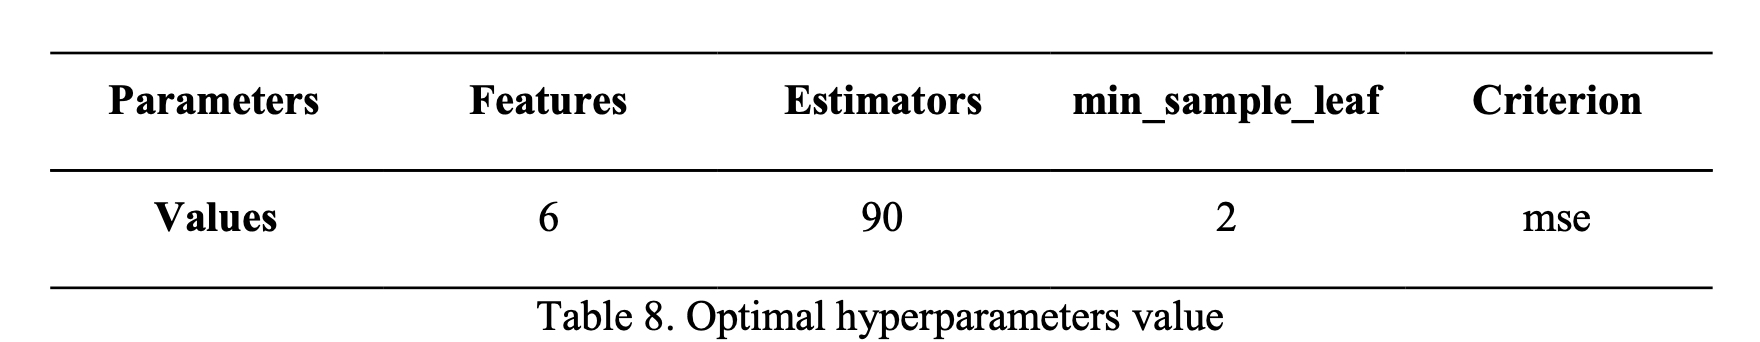
\includegraphics[width=4.45in,height=0.75in]{./media/image9.png}
	\end{Center}
\end{figure}


%%%%%%%%%%%%%%%%%%%% Figure/Image No: 6 Ends here %%%%%%%%%%%%%%%%%%%%

\par

\begin{Center}
{\fontsize{8pt}{9.6pt}\selectfont Table. 2 The optimal parameter of the random forest classifier\par}
\end{Center}\par

The confusion matrix of the logistic regression and result indicators are as follows.\par



%%%%%%%%%%%%%%%%%%%% Figure/Image No: 7 starts here %%%%%%%%%%%%%%%%%%%%

\begin{figure}[H]
	\begin{Center}
		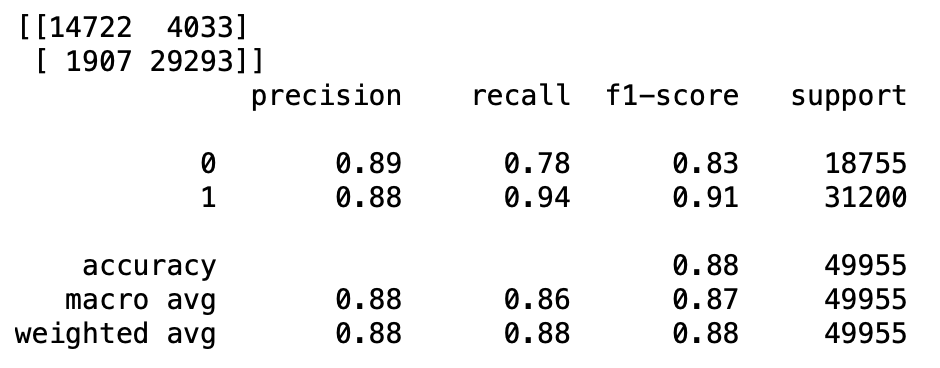
\includegraphics[width=3.72in,height=1.45in]{./media/image7.png}
	\end{Center}
\end{figure}


%%%%%%%%%%%%%%%%%%%% Figure/Image No: 7 Ends here %%%%%%%%%%%%%%%%%%%%

\par

\begin{Center}
{\fontsize{8pt}{9.6pt}\selectfont Figure. 4 Confusion matrix and results indicators of random forest classifier\par}
\end{Center}\par


\vspace{\baselineskip}
\textbf{3.3 Support Vector classifier}\par

The\ Support Vector Machine can also be used as a classification  method, maintaining all the main features that characterize the algorithm which is the maximal margin. There are several advantages that the SVR algorithm has, for instance, SVR model tends to have strong generalization ability and can reduce the probability of overfitting. There are several kernels in this model that needed to consider, they are as follows:\par

\begin{itemize}
	\item ●\  Linear Kernel\par

	\item ●\  Polynomial Kernel\par

	\item ●\  Radial-basis Function(RBF) Kernel\par

\setlength{\parskip}{12.0pt}
	\item ●\  Sigmoid Kernel
\end{itemize}\par

 In the support vector regression model, the RBF kernel is also known as the Gaussian Kernel, after we compared those four different kernels, we found out that the RBF kernel is the best fit for our model. And the formula for this kernel function is:\par

\begin{justify}
In this kernel function, we need to focus on two different hyperparameters, which is:
\end{justify}\par

\setlength{\parskip}{0.0pt}
\begin{itemize}
	\item ●\  C: Cost parameter of error item\par

\setlength{\parskip}{12.0pt}
	\item ●\  \textcolor[HTML]{222222}{Gamma:​ ​The parameter in the kernel function}
\end{itemize}\par

\begin{justify}
\textcolor[HTML]{222222}{In this model, in a gesture to avoid overfitting, we used the Cross Validation with k-ford equals 5 to find the optimal hyperparameters in the Support Vector Regression model. And the optimal hyperparameters we got based on the input of our training data. I firstly use default value to get the accuracy. Since the dataset is too large, then I use 2000 data and used in test data, get the accuracy about 85$\%$ . Then I use heat map to find the optimal parameter based on different C and gamma and choose kernel as ‘RBF’.}
\end{justify}\par



%%%%%%%%%%%%%%%%%%%% Figure/Image No: 8 starts here %%%%%%%%%%%%%%%%%%%%

\begin{figure}[H]
	\begin{Center}
		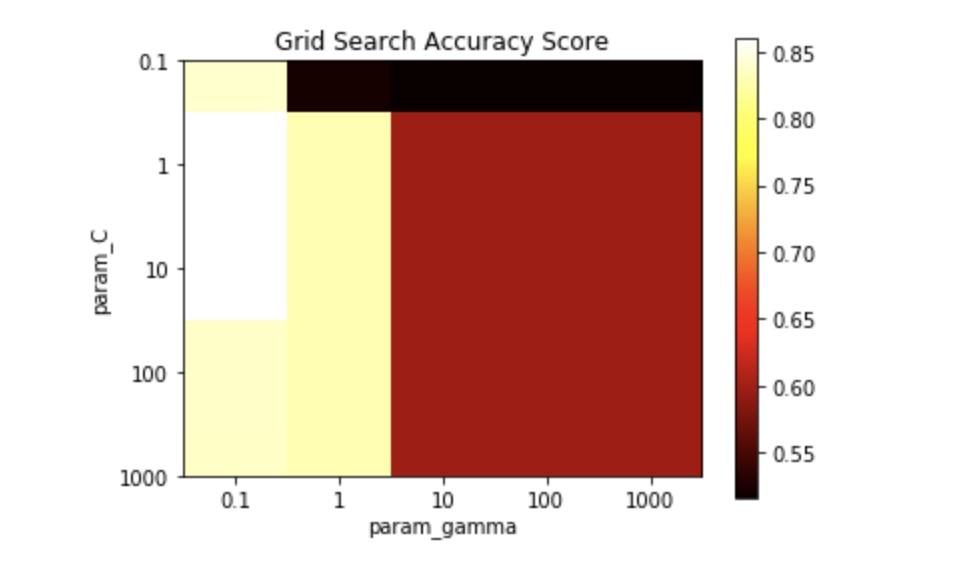
\includegraphics[width=4.44in,height=2.6in]{./media/image6.jpg}
	\end{Center}
\end{figure}


%%%%%%%%%%%%%%%%%%%% Figure/Image No: 8 Ends here %%%%%%%%%%%%%%%%%%%%

\par

\begin{Center}
{\fontsize{8pt}{9.6pt}\selectfont Figure.5 Heat map for different parameter(C, gamma)\par}
\end{Center}\par

\begin{justify}
\textcolor[HTML]{222222}{We could see that the C equals to 10 and gamma equals to 0.1, getting the accuracy about 87.3$\%$ }
\end{justify}\par


\vspace{\baselineskip}
\textbf{3.4 Gaussian Naive Bayes classifier}\par

\begin{justify}
\textcolor[HTML]{222222}{A Naive Bayes classifier is a probabilistic machine learning model that’s used for classification task. The crux of the classifier is based on the Bayes theorem.}
\end{justify}\par

\begin{justify}
\textcolor[HTML]{222222}{The confusion matrix of the logistic regression and result indicators are as follows.}
\end{justify}\par


\vspace{\baselineskip}


%%%%%%%%%%%%%%%%%%%% Figure/Image No: 9 starts here %%%%%%%%%%%%%%%%%%%%

\begin{figure}[H]
	\begin{Center}
		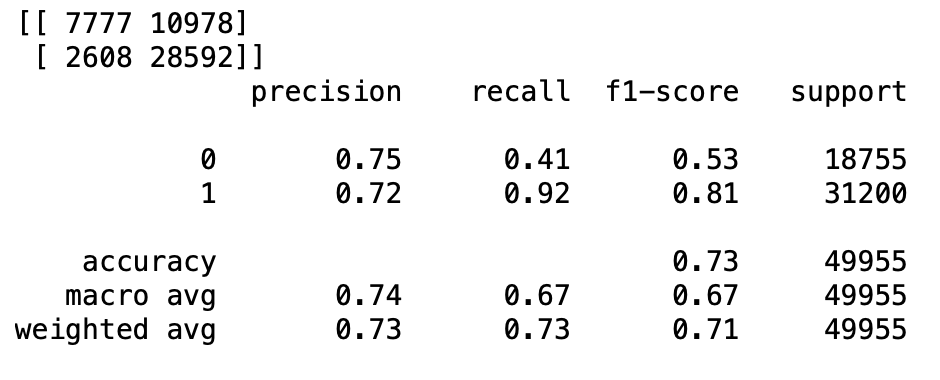
\includegraphics[width=3.48in,height=1.41in]{./media/image8.png}
	\end{Center}
\end{figure}


%%%%%%%%%%%%%%%%%%%% Figure/Image No: 9 Ends here %%%%%%%%%%%%%%%%%%%%

\par

\begin{Center}
{\fontsize{8pt}{9.6pt}\selectfont Figure.6 Confusion matrix and results indicators of gaussian naive bayes\par}
\end{Center}\par


\vspace{\baselineskip}
\textbf{3.5 Model effectiveness comparison}\par

\begin{justify}
From the bar plot, we can observe the logistic regression has a better performance on the H-1B Visa Petitions 2011-2016 dataset with prediction accuracy of 89.1$\%$ 
\end{justify}\par



%%%%%%%%%%%%%%%%%%%% Figure/Image No: 10 starts here %%%%%%%%%%%%%%%%%%%%

\begin{figure}[H]
	\begin{Center}
		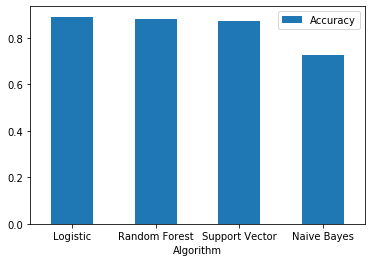
\includegraphics[width=3.88in,height=2.73in]{./media/image5.png}
	\end{Center}
\end{figure}


%%%%%%%%%%%%%%%%%%%% Figure/Image No: 10 Ends here %%%%%%%%%%%%%%%%%%%%

\par

\begin{Center}
{\fontsize{8pt}{9.6pt}\selectfont Figure.7 Prediction accuracy comparison \par}
\end{Center}\par

{\fontsize{14pt}{16.8pt}\selectfont \textbf{4. Conclusion}\par}\par


\vspace{\baselineskip}
\begin{justify}
\textbf{4.1 Weapon of Math Destruction}
\end{justify}\par

\begin{justify}
There is no significant factors that suggest that our project is a weapon of math destruction(WMD). The purpose of this model is used for visa applicant’s reference and help applicants better arrange their future work plan but not used for USCIS decision procedure of the visa. All the features in our dataset are extracted from ETA forms(employer’s labor condition applications) from U.S. Department of Labor and are important factors of government’s consideration of the visa application outcomes. The modeling process is static and unidirectional (using relevant government information to predict the approval outcome) with no feedback loop impact. The predictions are only for reference purposes so it is hard to infer any damaging effect to the society. Therefore, our project can’t have negative implications on large numbers of people. 
\end{justify}\par


\vspace{\baselineskip}
\begin{justify}
\textbf{4.2 Fairness}
\end{justify}\par

\begin{justify}
There is no significant fairness concern in this project. On the one hand, the features in our dataset are nominal or numerical values reflecting information about employment status and geographic location. These features reflecting objective information about the applicant’s working ability and potential value for the sponsor company. Actually, companies tend to recognize their employees’ value when they are willing to help the employee applying for H-1 visa. Therefore, Most of the applicants in the dataset are competitive candidates. There is no unfairness concern in the dataset. On the other hand, because we are preprocessing each feature and evaluating them by the same methods to make predictions, there should be no apparent discrimination associated with our prediction models.
\end{justify}\par


\vspace{\baselineskip}
\begin{justify}
\textbf{4.3 Summary and potential improvement}
\end{justify}\par

\begin{justify}
Using techniques[4] we learned in class(K-fold cross validation, logistic regression, support vector machines) and also some other techniques learned outside(random forest), we were able to find models that can predict whether one will experience denied or approved for the H1B application given the dataset we used. 
\end{justify}\par

\begin{justify}
We\ do feel confident that our results can be used in production to see whether one will be denied based on the dataset information.  Our project results can be used by government or non-profit agencies to help predict the people such that non-native students in america have the opportunities to work here and start preparing to be higher probabilities to be approved such like working in some information science related job or find the bigger company like google. In the future, there is potential to add more features to help increase the accuracy. 
\end{justify}\par


\vspace{\baselineskip}
{\fontsize{14pt}{16.8pt}\selectfont \textbf{5. Reference}\par}\par

\setlength{\parskip}{0.0pt}
[1] https://webpages.uncc.edu/sshinde5/\par

\setlength{\parskip}{12.0pt}
[2] K.-Luckyson, S. Saha, and S-R.Dey, $``$Predicting the direction of stock market prices using random forest$"$  ​\textit{Applied Mathematical Finance}​, 2016.\par

[3] C.Y.Yeh, C-W. Huang, and Shie-J.Lee, $``$A multiple-kernel support vector regression approach for a stock market price forecasting,$"$  ​\textit{Science Direct.},​ 2010.\par

\setlength{\parskip}{0.0pt}
[4] Andrew NG, $``$Machine Learning, Stanford University course$"$ .\par


\printbibliography
\end{document}